\documentclass[aspectratio=169]{beamer}
\usetheme[titleformat title=smallcaps]{metropolis}

% Configure Theme
% Disable separate dark color for frame titles
\setbeamercolor{frametitle}{fg=normal text.fg, bg=normal text.bg}

% More padding for frame titles. Align with text body.
\makeatletter
\setlength{\metropolis@frametitle@padding}{3ex}
\setbeamersize{text margin left=3ex, text margin right=3ex}
\makeatother

% Reveal slides on a frame gradually, used with \pause, \uncover or \onslide
\setbeamercovered{dynamic}

% Fonts
% \usepackage{fontspec}  % Requires LuaLaTeX
% \usepackage{mathtools}  % Math
% \usepackage[
%   warnings-off={
%       mathtools-colon,%
%       mathtools-overbracket,%
%     }
% ]{unicode-math}% Load after mathtools
% \usepackage[tracking]{microtype}

% \setmainfont[Numbers=Lowercase]{TeX Gyre Pagella}
% \setmonofont[AutoFakeSlant,Scale=MatchLowercase]{inconsolata}
% \setsansfont{Merriweather Sans}
% \setmathfont[mathrm=sym,mathit=sym,mathsf=sym,mathbf=sym,mathtt=sym,NFSSFamily=tgpl]{TeX Gyre Pagella Math}
% \newfontfamily{\unitnumberfont}[Numbers=Uppercase]{TeX Gyre Pagella}
% \usefonttheme{serif}
% \setbeamerfont to define fonts used e.g. in heading, block , footer, ...

% Additional packages
\usepackage{siunitx}
\usepackage{appendixnumberbeamer} % To make the appendix into backup slides
\usepackage{fontawesome5}

\title{Building a 25 MHz NMR Spectrometer}
\date{\today}
\author{Maximilian Stabel}
\institute{ETH Zürich}

% TODO:
% - Make same style as thesis, e.g.
%   - Font
%   - ETH Color Scheme
% - align column left with heading/rest of text

\begin{document}
\maketitle
% \section{First Section}
\begin{frame}{Our goal is a functioning low-field\\NMR benchtop spectrometer}
  \begin{figure}
    \centering
    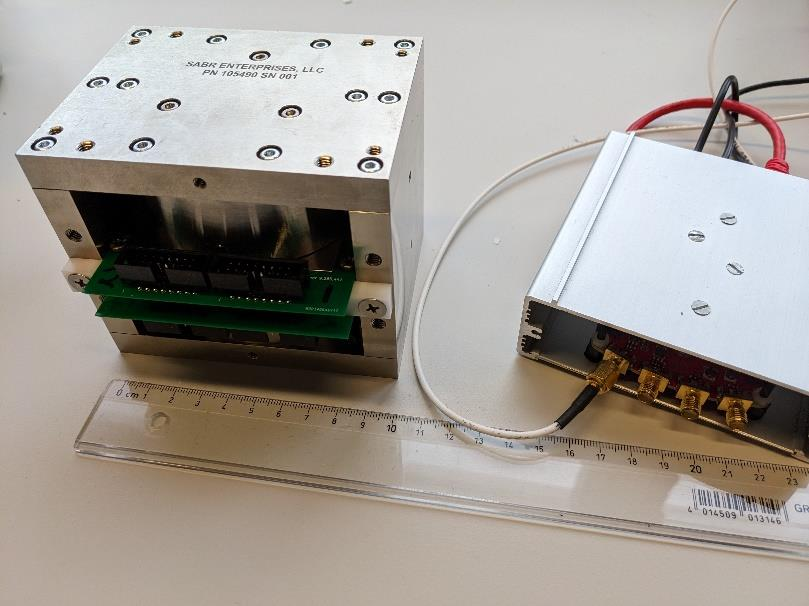
\includegraphics[width=\textwidth,height=0.8\textheight,keepaspectratio]{./img/magnet.png}
  \end{figure}
\end{frame}
\begin{frame}{We've made a probe holder\\and an RF-coil already}
  \begin{columns}
    \begin{column}{0.45\textwidth}
      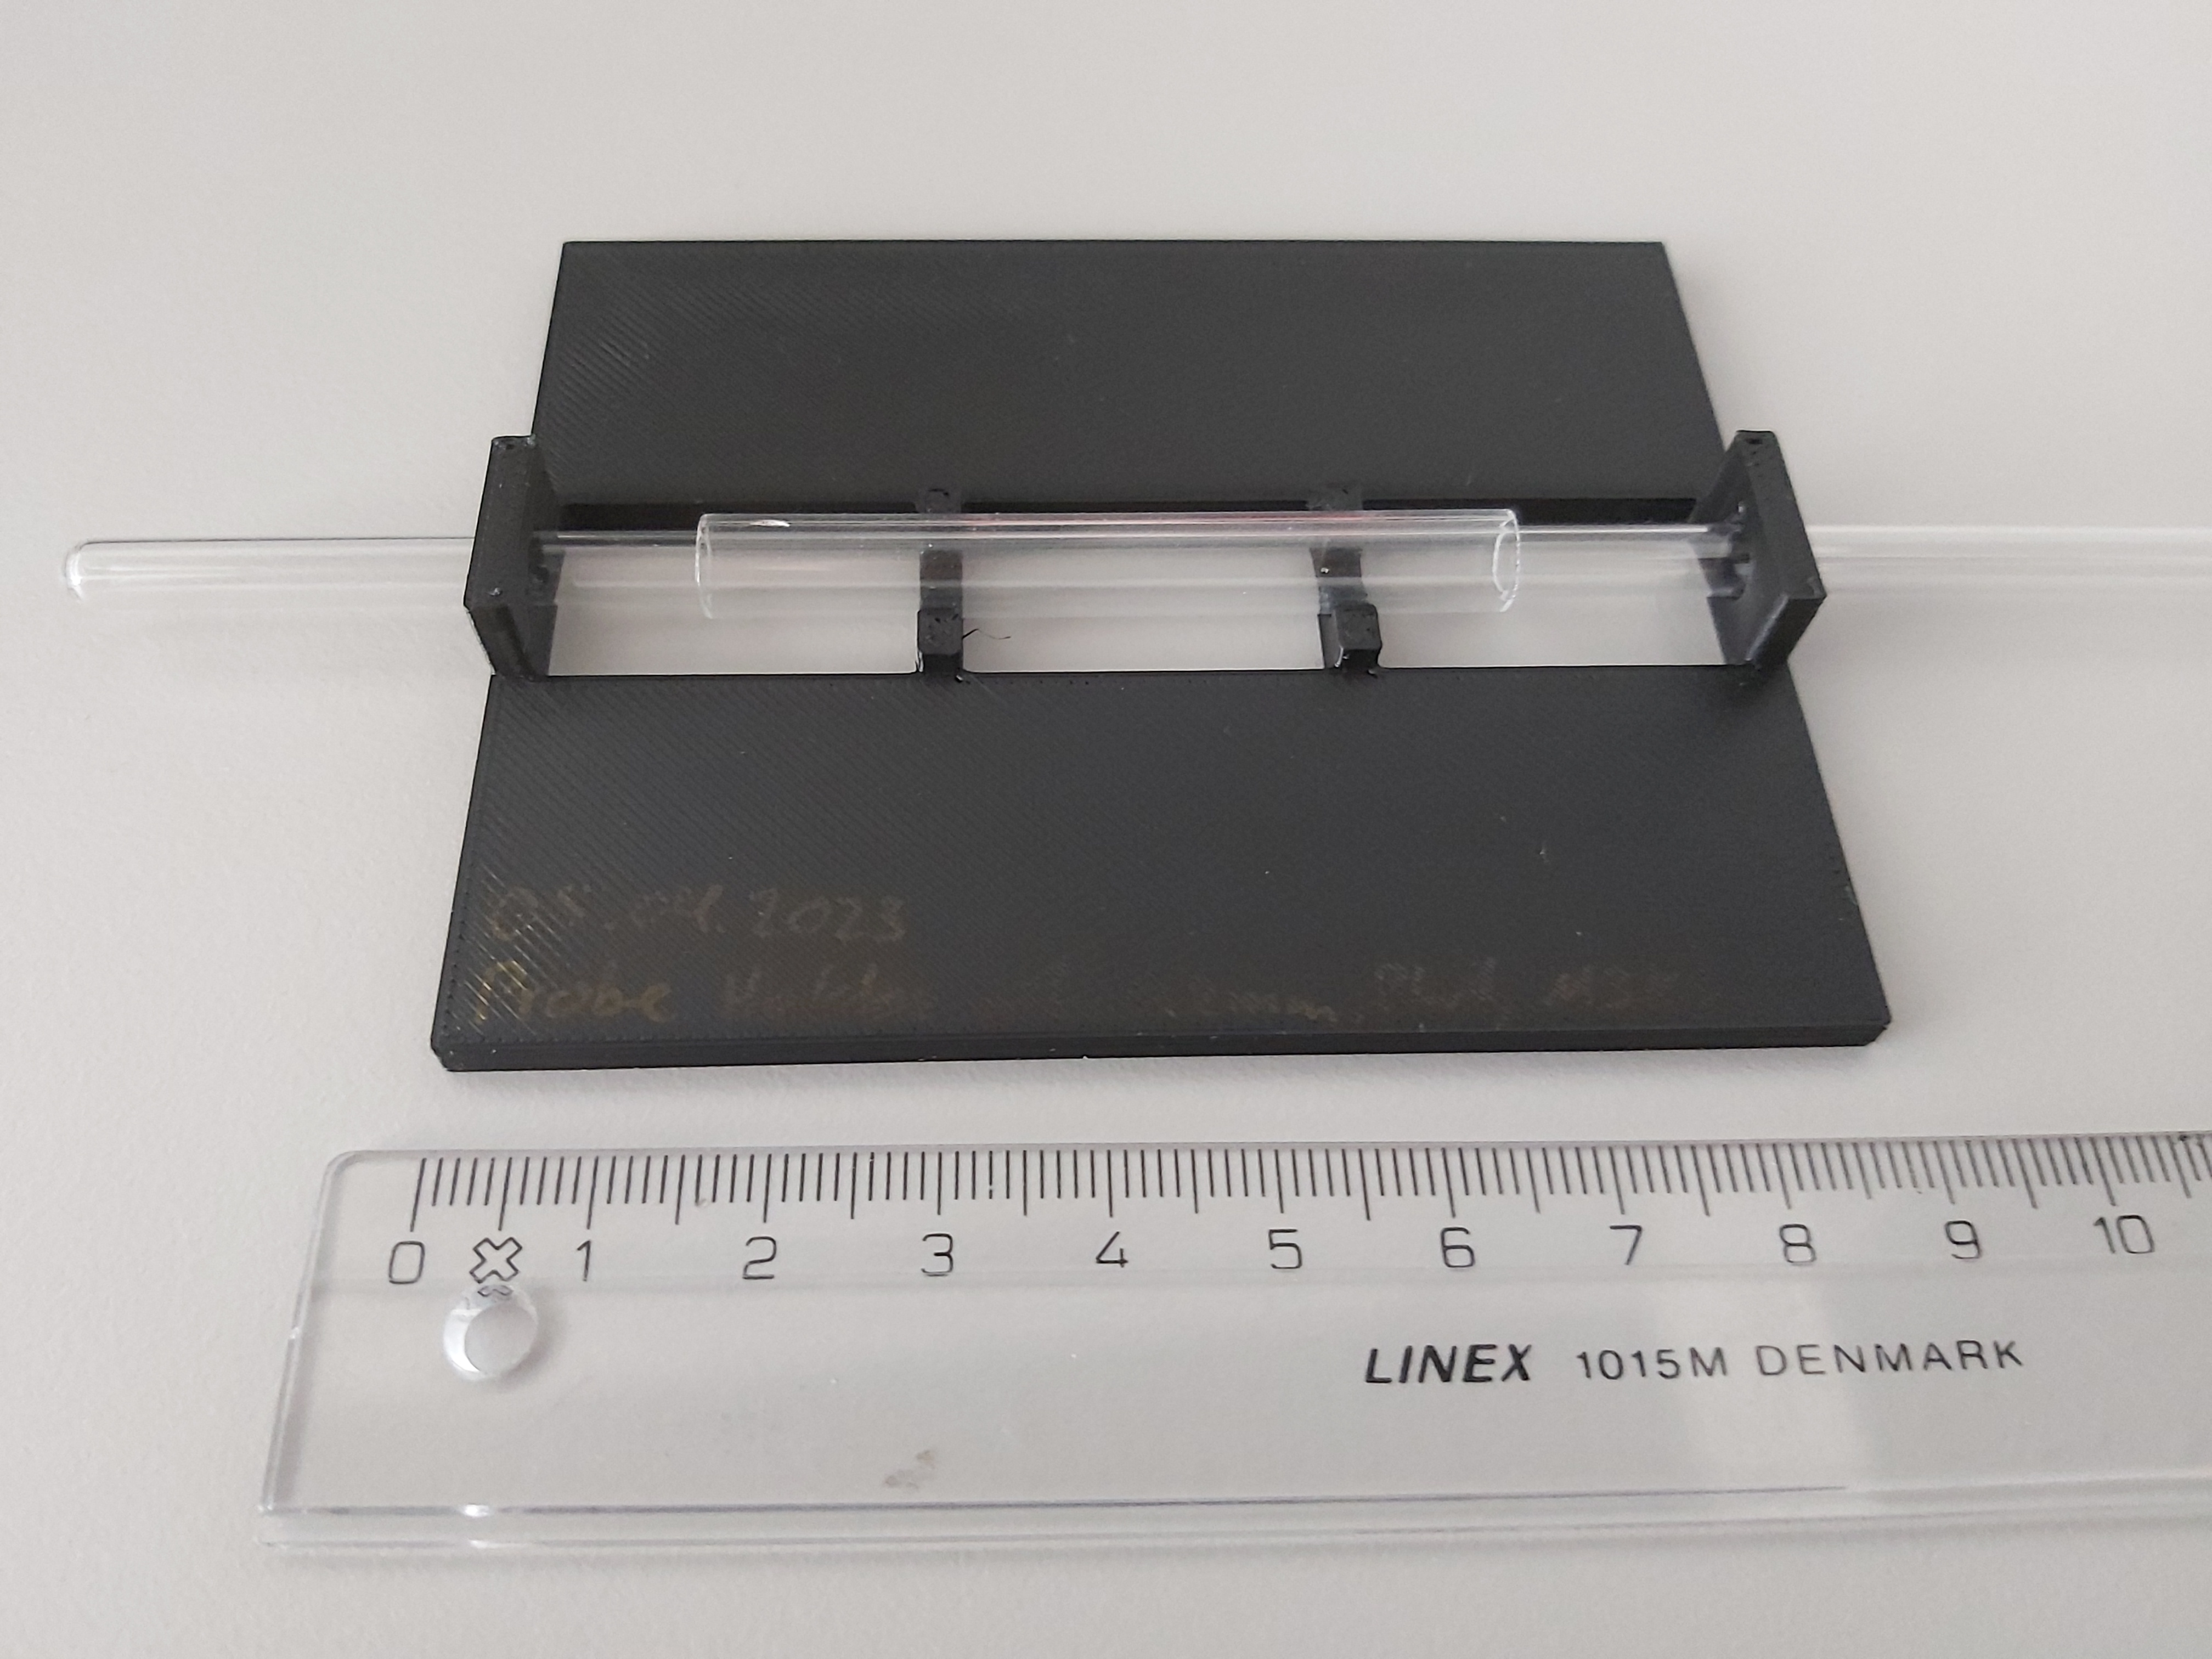
\includegraphics[width=\textwidth]{./img/probe_holder.jpg}
    \end{column}
    \begin{column}{0.45\textwidth}
      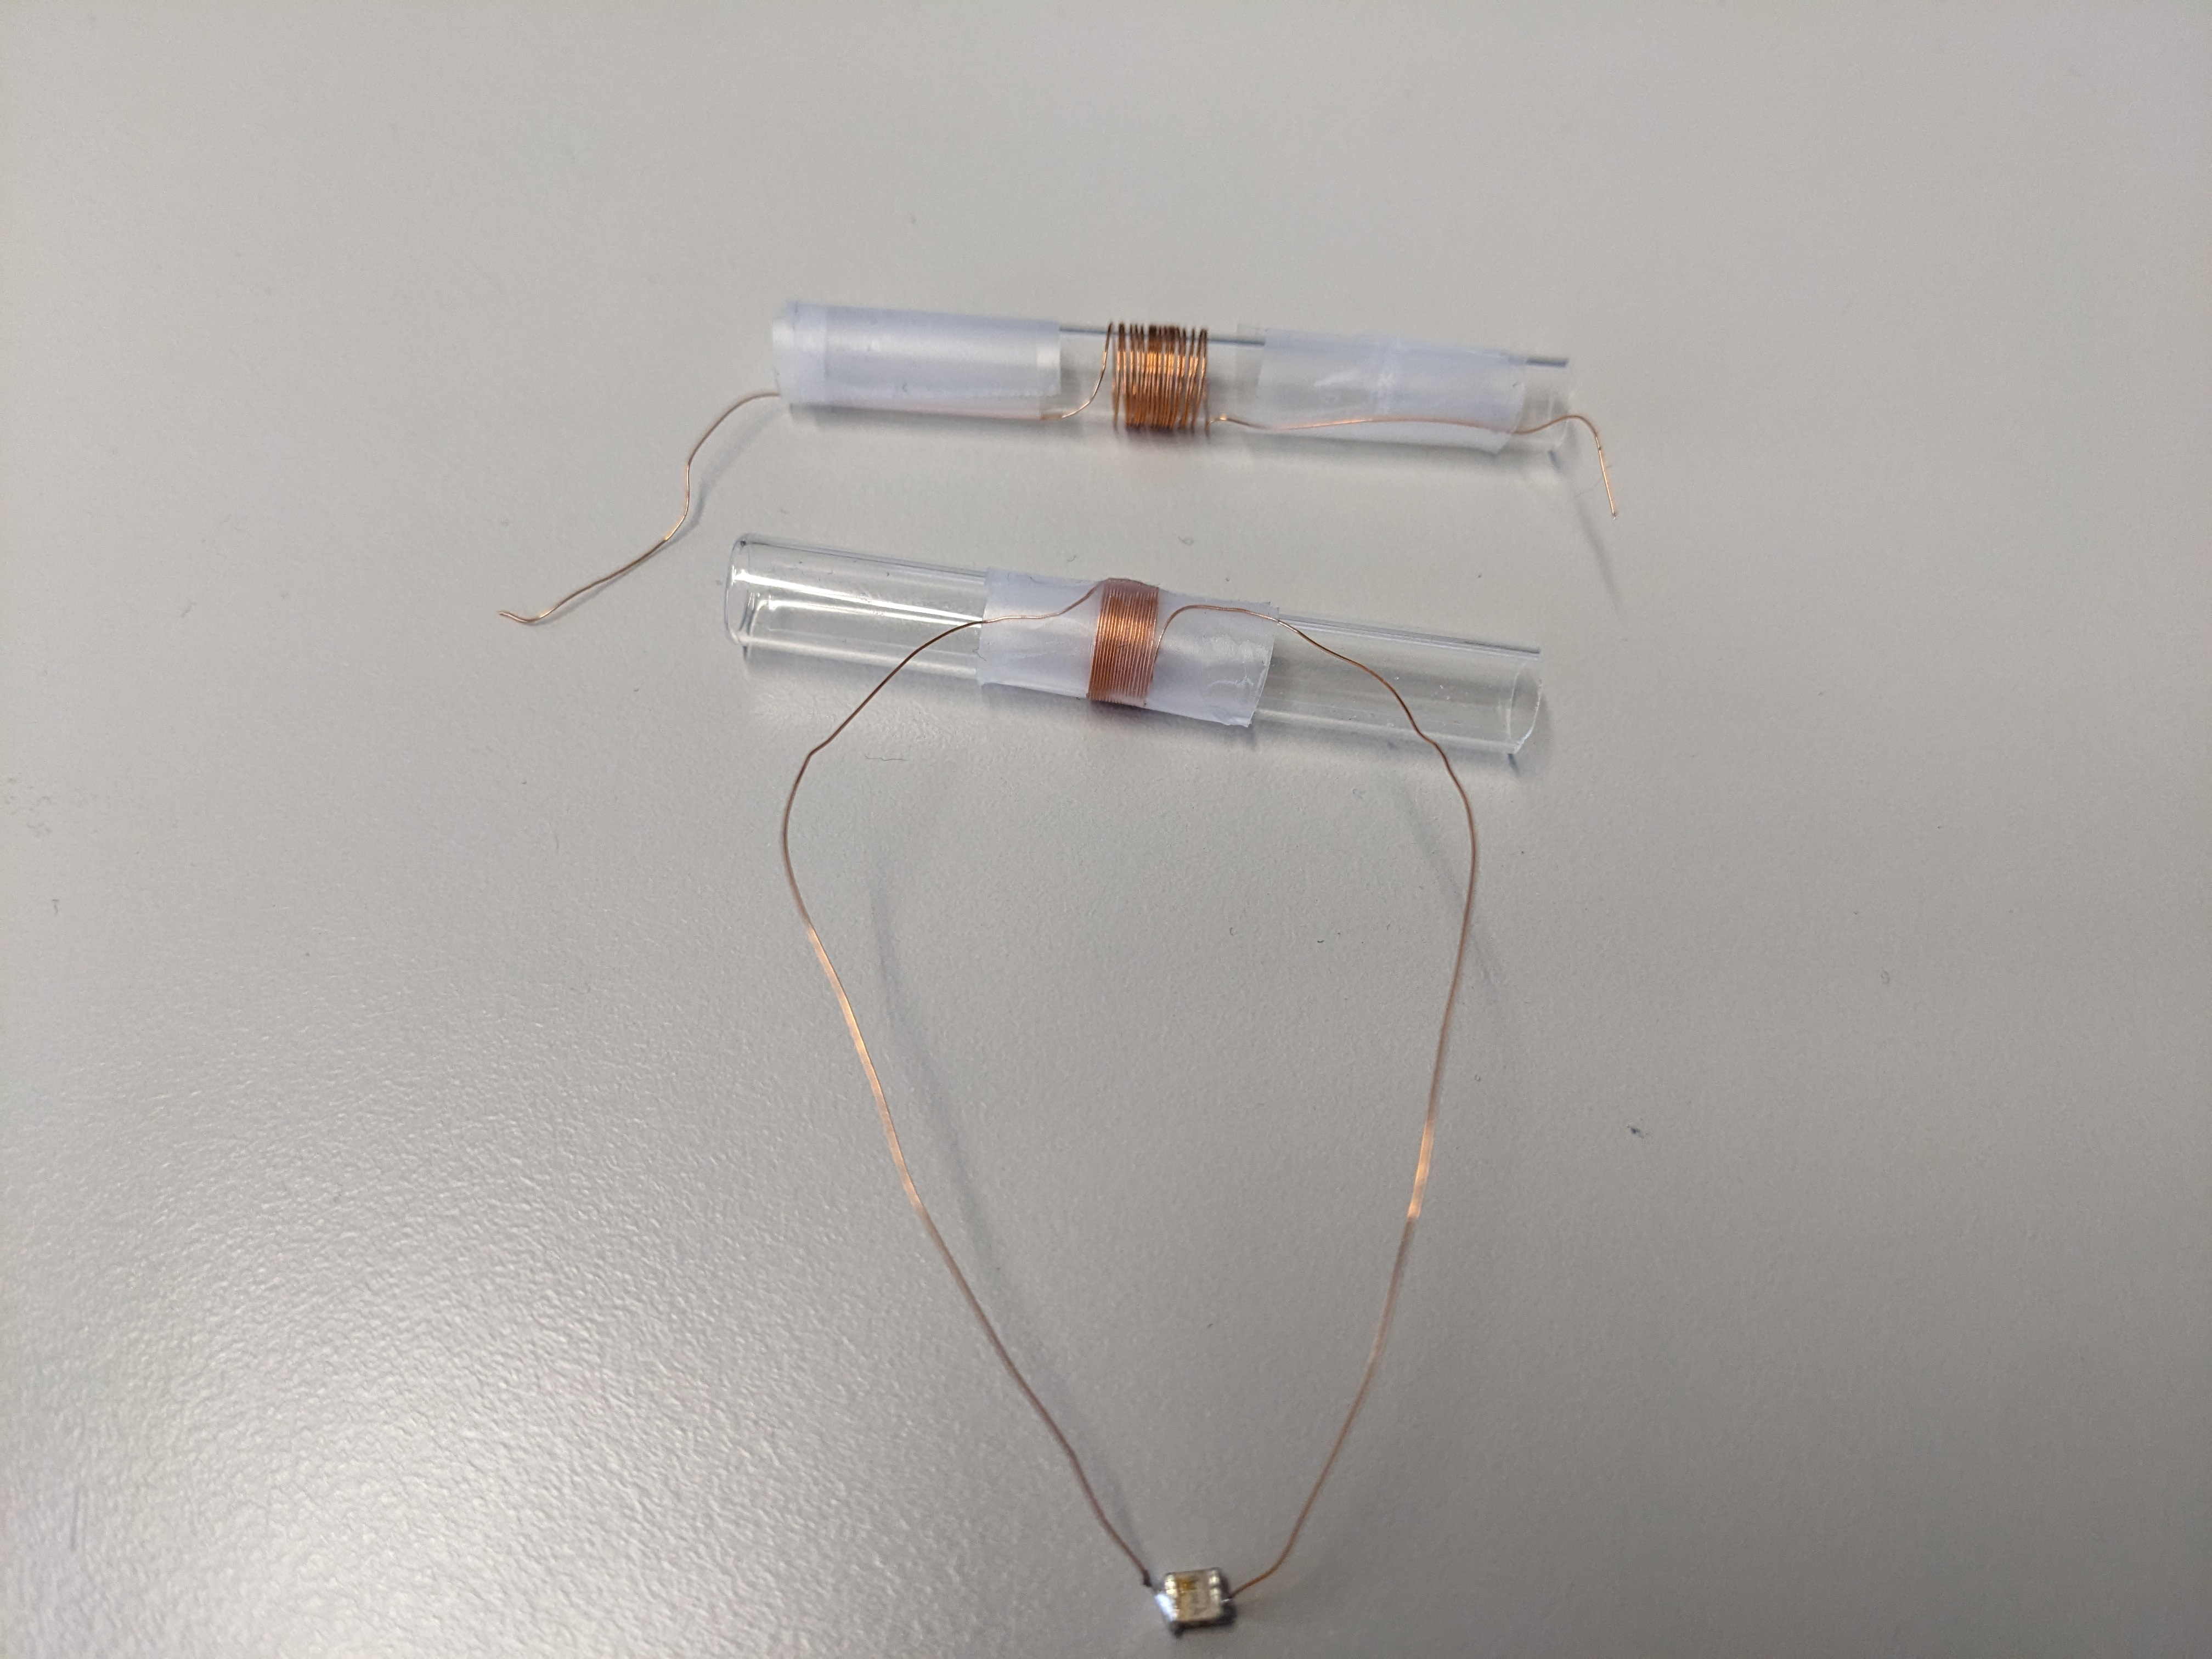
\includegraphics[width=\textwidth]{./img/coil.jpg}
    \end{column}
  \end{columns}
\end{frame}
\begin{frame}{Next we will setup the console, measure the magnetic field\\and build, match and tune the probe}
  \begin{columns}
    \begin{column}{0.33\textwidth}
      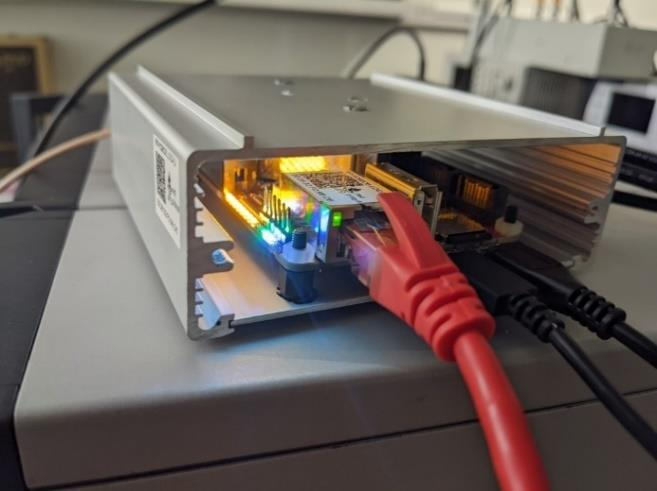
\includegraphics[width=\textwidth, height=0.8\textheight, keepaspectratio]{./img/red_pitaya.png}
    \end{column}
    \begin{column}{0.33\textwidth}
      \centering
      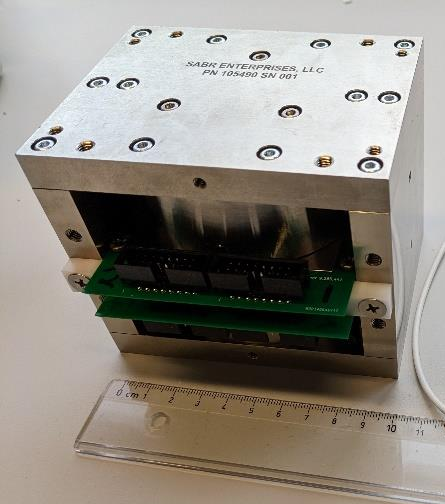
\includegraphics[width=\textwidth, height=0.8\textheight, keepaspectratio]{./img/magnet_only.png}
    \end{column}
    \begin{column}{0.33\textwidth}
      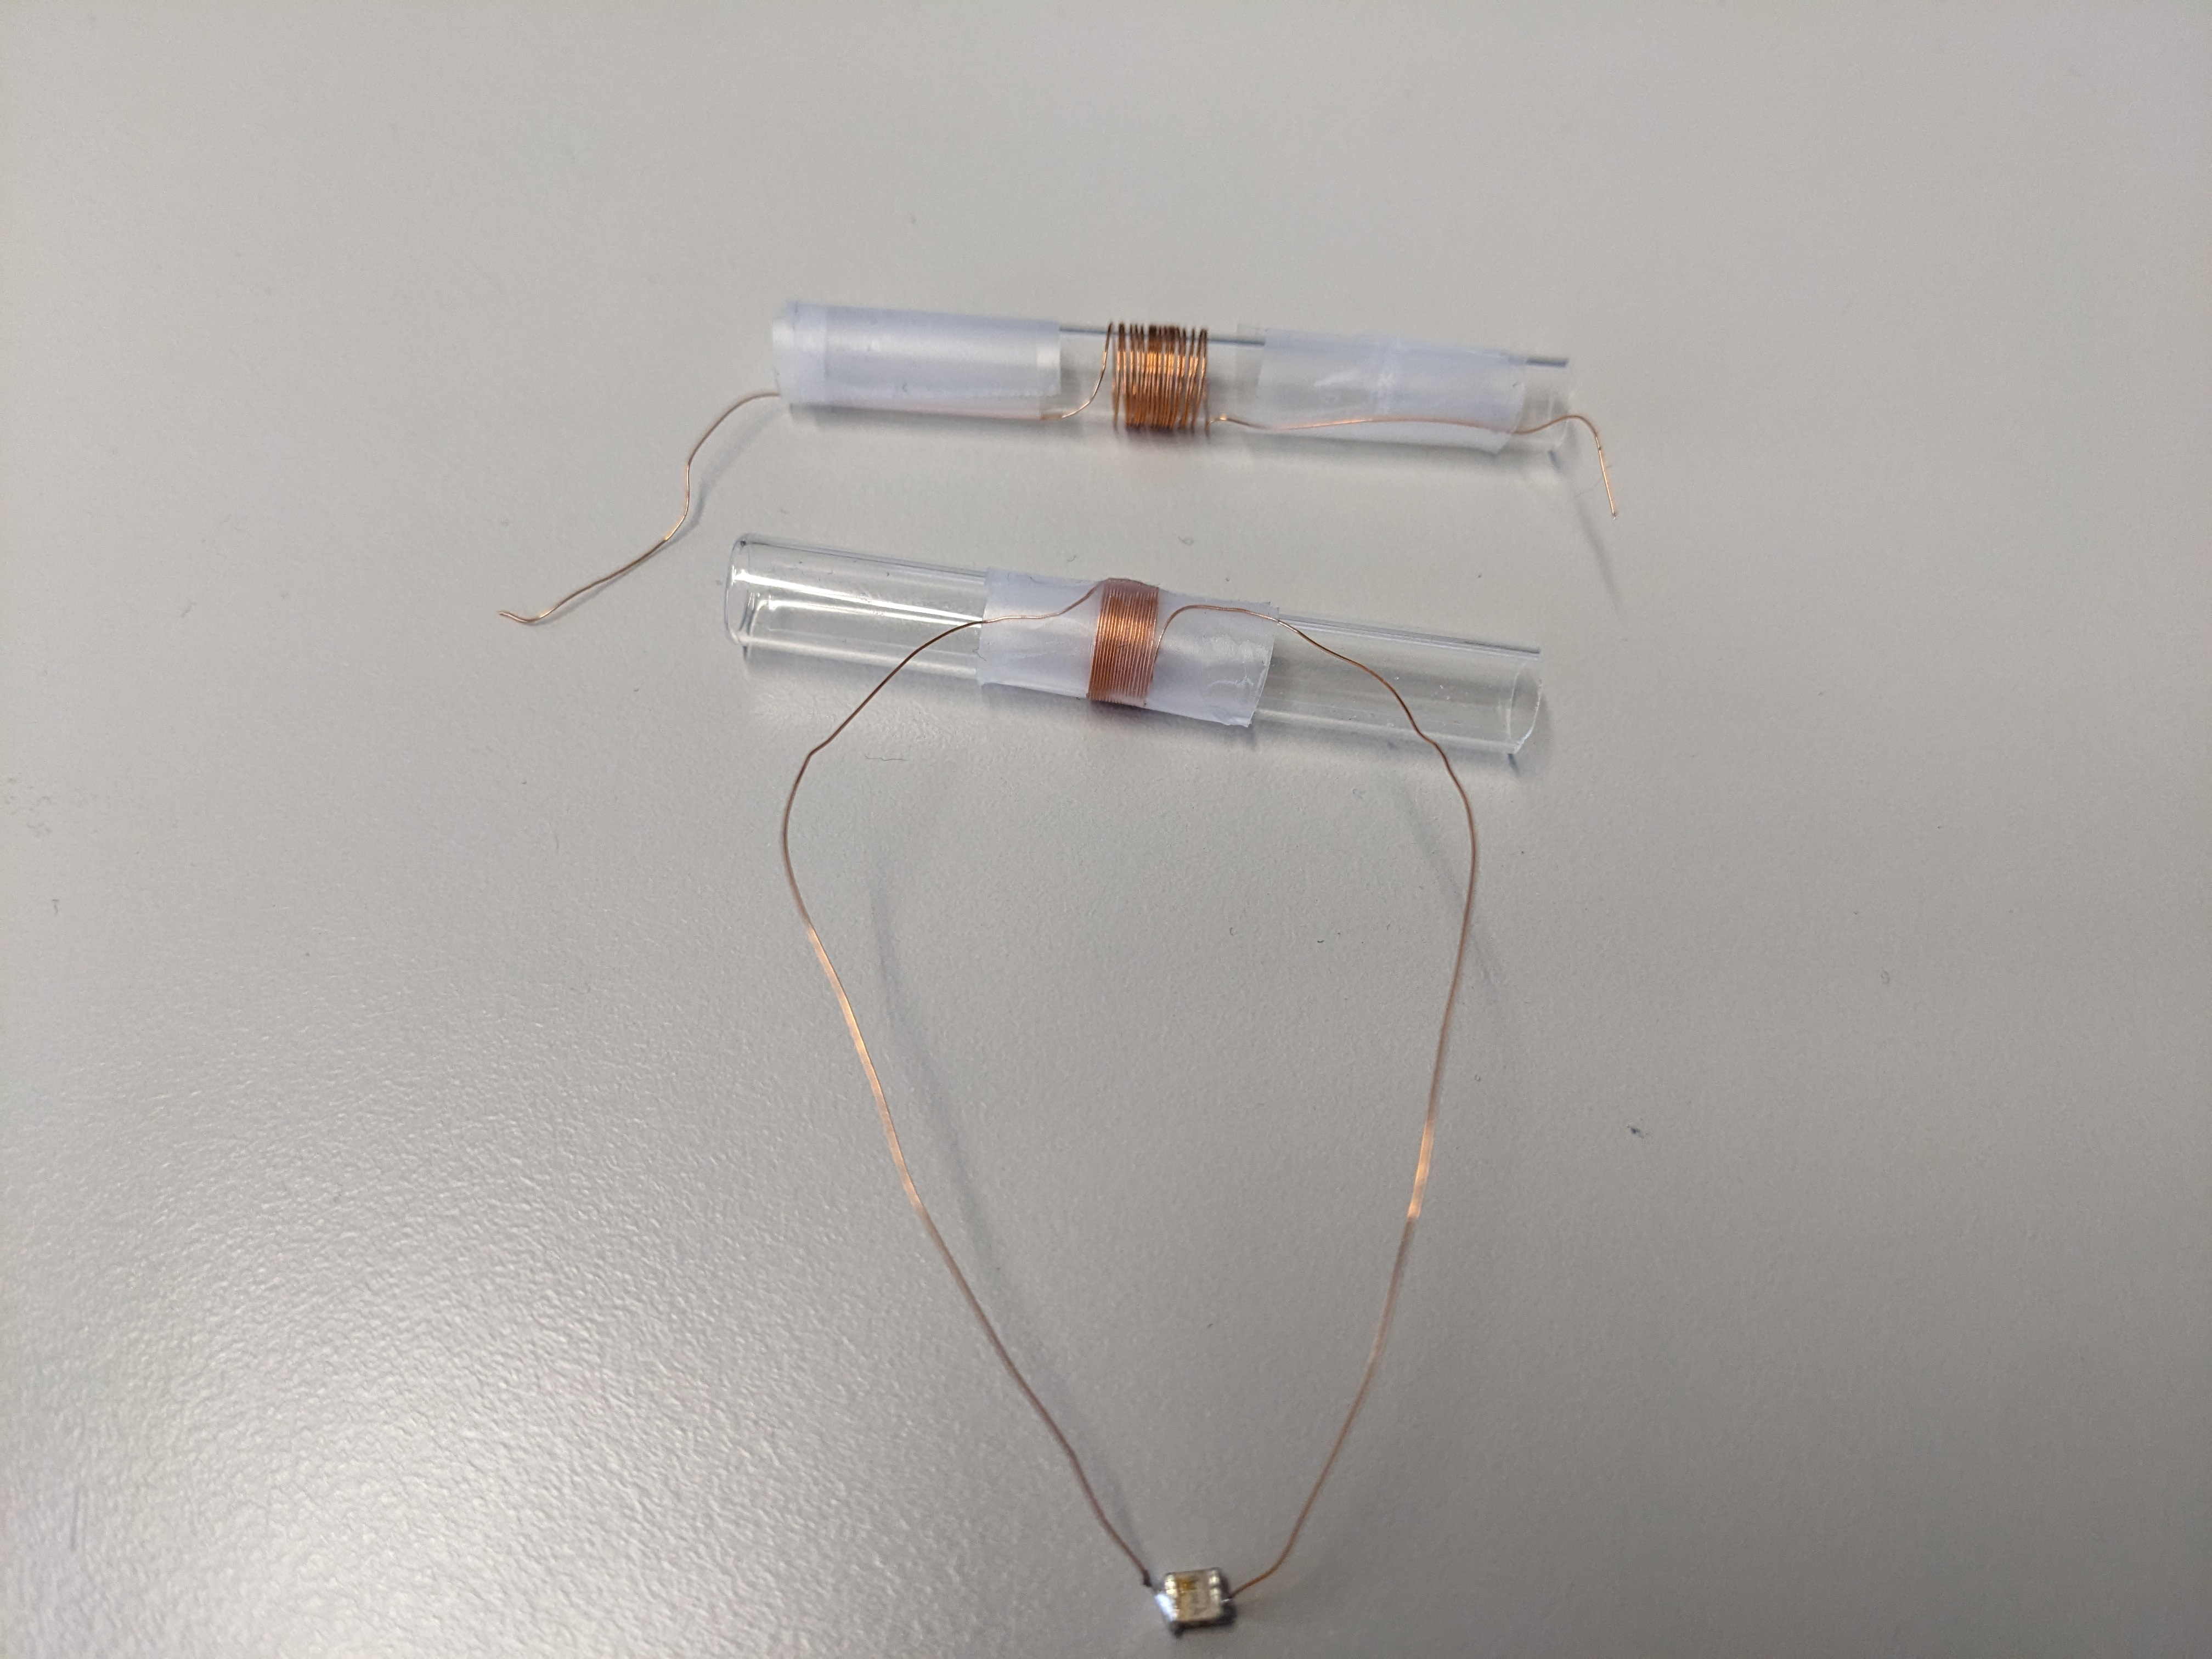
\includegraphics[width=\textwidth, height=0.8\textheight, keepaspectratio]{./img/coil.jpg}
    \end{column}
  \end{columns}
\end{frame}
\begin{frame}[standout]
  Thank you!
\end{frame}
\appendix
% \begin{frame}[standout]
%   A backup graph for explaining things.
% \end{frame}
\end{document}